\chapter{Introduction}
\label{sec:introduction}

People often sketch when solving problems.  Some sketches are
personal; others are collaborative. Some sketches help people make
quick calculations and are quickly forgotten; others serve longer-term
purposes. For professional designers, sketching serves as a means for
thinking about problems as much as it does for communicating proposed
solutions. For people who are not designers, sketching is a natural
means for quickly recording spatial information such as directions to
a point of interest.

Design can be seen as an iterative process of problem-framing and
exploring possible solutions within the current conception of the
problem. Sketching allows people to visually represent ideas quickly,
without prematurely committing to decisions. A sketch is not a
contract: it is a proposal that can be modified, erased, built
upon. The rough look of hand-made sketches suggests their provisional
nature.

Some theories of cognition give the human mind two distinct tasks: to
perceive the world via our senses, and to reason about what our senses
provide. In contrast, the late psychologist Rudolf Arnheim argues that
perception and thinking are inseparable: ``Unless the stuff of the
senses remains present the mind has nothing to think
with''~\cite{arnheim-visthink}. Visual thinking is valuable in
evaluating what is and designing what might be. Sketching allows
people to give form to notions that are otherwise imaginary; the act
of seeing fuels the process of reasoning.

The term ``sketch'' is used in many ways in vernacular and academic
work. Some speak of sketching as a process---we sketch out an idea by
talking about it, drawing pictures, or play-acting while considering
possible solutions or problem formulations. Alternately we may use the
term ``sketch'' to mean the product of an exploration, as when we make
a prototype out of modeling clay, cardboard, or code.

In this survey we define a \textit{sketch} based on the utility
hand-made drawings afford: sketches are quickly made depictions that
facilitate visual thinking. In this way, sketches may include
everything from doodles to roughly drawn circuit diagrams to an
architect's quick isometric projection. We restrict neither the
drawing medium nor the subject matter. Sketches are most often
two-dimensional graphic depictions, but often incorporate textual
annotations.

Sketching has been a topic of interest to computer scientists and HCI
practitioners for quite some time. Early efforts such as
Sketchpad~\cite{sutherland-sketchpad} and GRAIL~\cite{ellis-grail}
hinted at the potential of pen based interfaces. In fact, many of
today's sketch-related research challenges were suggested by these
systems 45 years ago.

Recently there has been a recurrence of interest in supporting
sketching with computation. Computers can recognize user input and let
people interact with drawings in ways that are impossible with paper
alone, augmenting the sketching process in various ways. A rough
sketch may contain enough information to infer the user's
intentions. The drawing could then come alive, for example providing a
simulation. Alternately the user's sketch may serve as a search
query. Beyond recognition, a computer can render, rectify, or beautify
a user's sketchy input into some other representation. Computation
also supports editing operations that are impossible with physical
sketches, for example enabling collaborators in different locations to
share an electronic drawing surface.

Researchers from many disciplines have contributed to knowledge about
sketching and computational techniques for supporting it. Their
diversity makes it difficult to get a complete sense of what has been
done on this topic. This review draws from journals, conference
proceedings, symposia and workshops in human-computer interaction,
cognitive science, design research, computer science, artificial
intelligence, and engineering design. These fields certainly overlap;
however research in sketching lacks a unifying publication venue.

Some who study sketching as an element of design practice publish in
the \textit{Design Studies} journal. Sketching has become a recurring
theme at HCI conferences like CHI, UIST, IUI and AVI, and visual
languages conferences such as IEEE's VL and VL/HCC. The Association
for the Advancement of Artificial Intelligence (AAAI) held symposia on
diagrammatic representation and reasoning~\cite{glasgow-diagrams} and
sketch understanding. The community brought together by the AAAI
sketch understanding symposia continues meeting at the annual
Eurographics Sketch Based Interaction and Modeling workshop
(SBIM). Related work has been published in computer graphics venues
such as \textit{Computers \& Graphics} and the Non-Photorealistic
Animation and Rendering conference.  There is also a substantial
amount of work published in various journals for electrical,
mechanical, or software engineering.

Surprisingly, few surveys on sketch recognition and interaction have
been published. Readers interested in pen computing in general may
find Meyers' earlier review helpful~\cite{meyer-pen-review}. That
survey covers pen-related hardware, handwriting recognition, and
presents a brief history of the traditional and computational use of
pens but only briefly mentions sketching. Ward has compiled an online
annotated bibliography of pen computing references that spans most of
the 20$^{th}$ century~\cite{ward-pen-bibliography}.

\section{A brief history of pen and sketching systems}
\label{sec:intro-brief-history}

\begin{figure}[]
   \centering
   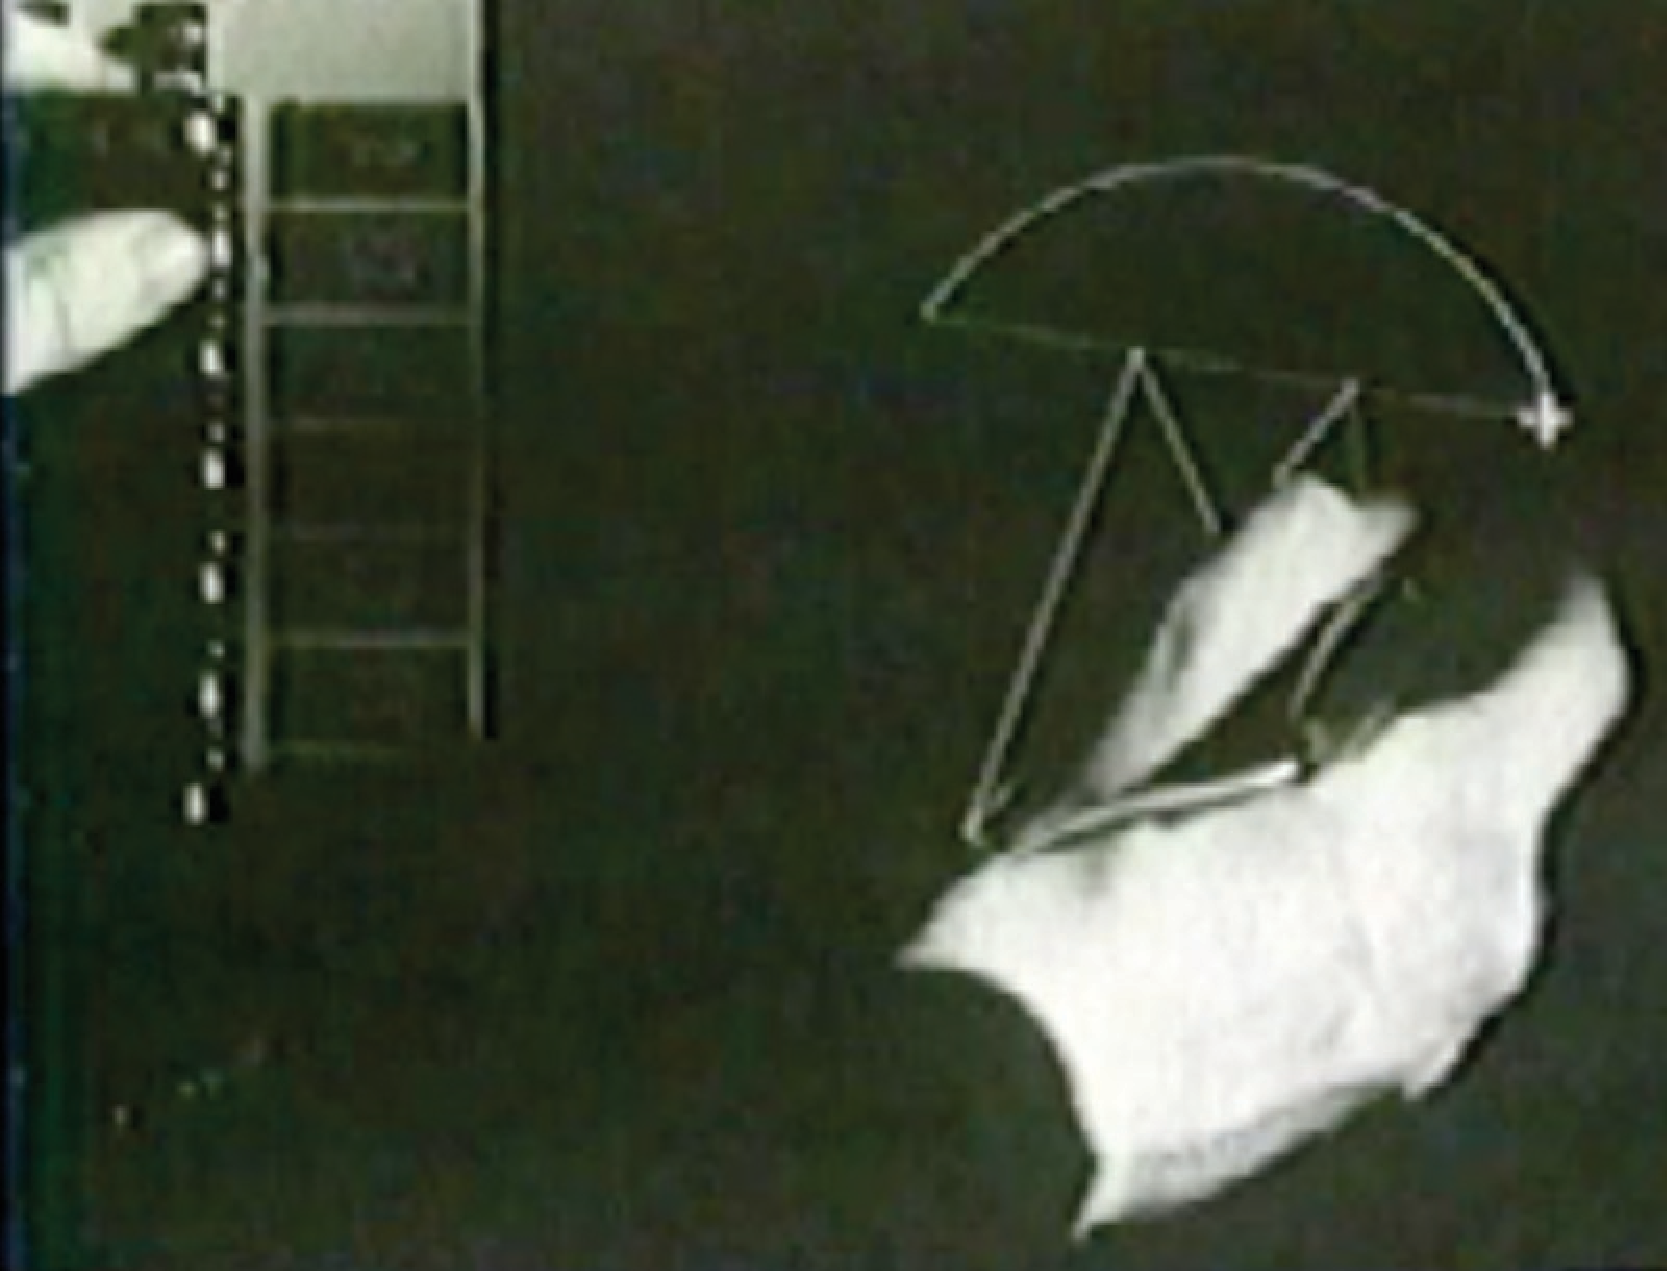
\includegraphics[width=3in]{img/sketchpad.pdf} 
   \caption{Sketchpad supported users in creating design drawings
     using pen input (right hand) and constraints (specified by
     buttons aligned vertically at left).}
   \label{fig:sketchpad}
\end{figure}

Sketchpad was the first to demonstrate many techniques in computer
science, human-computer interaction, and computational
design~\cite{sutherland-sketchpad}. It was an interactive design
system allowing an engineer to create models by drawing with a light
pen on a graphical display. The user could apply constraints (such as
``make this line parallel to that line and maintain that relation'')
that relieved the burden of manually maintaining such
relations. Figure~\ref{fig:sketchpad} shows the user defining the
shape of a rivet through a combination of drawing and constraint
specification.

RAND's GRAIL system (GRAphical Input Language) interpreted stylus
input in a particular visual programming language for creating control
sequence flowcharts~\cite{ellis-grail}. GRAIL allowed users to quickly
specify these programs graphically, rather than textually. To provide
input, users drew or wrote freely on a digitizing tablet. GRAIL then
attempted recognition using domain and contextual information to
determine what the input meant (see Figures~\ref{fig:grail-box} and~\ref{fig:grail-gesture}). The user could add semantically meaningful
model data (boxes, arrows, writing) and issue commands (erase a line,
move a box, change the data type of a node) without explicitly
entering a mode.

\begin{samepage}
\begin{figure}
\begin{center}
  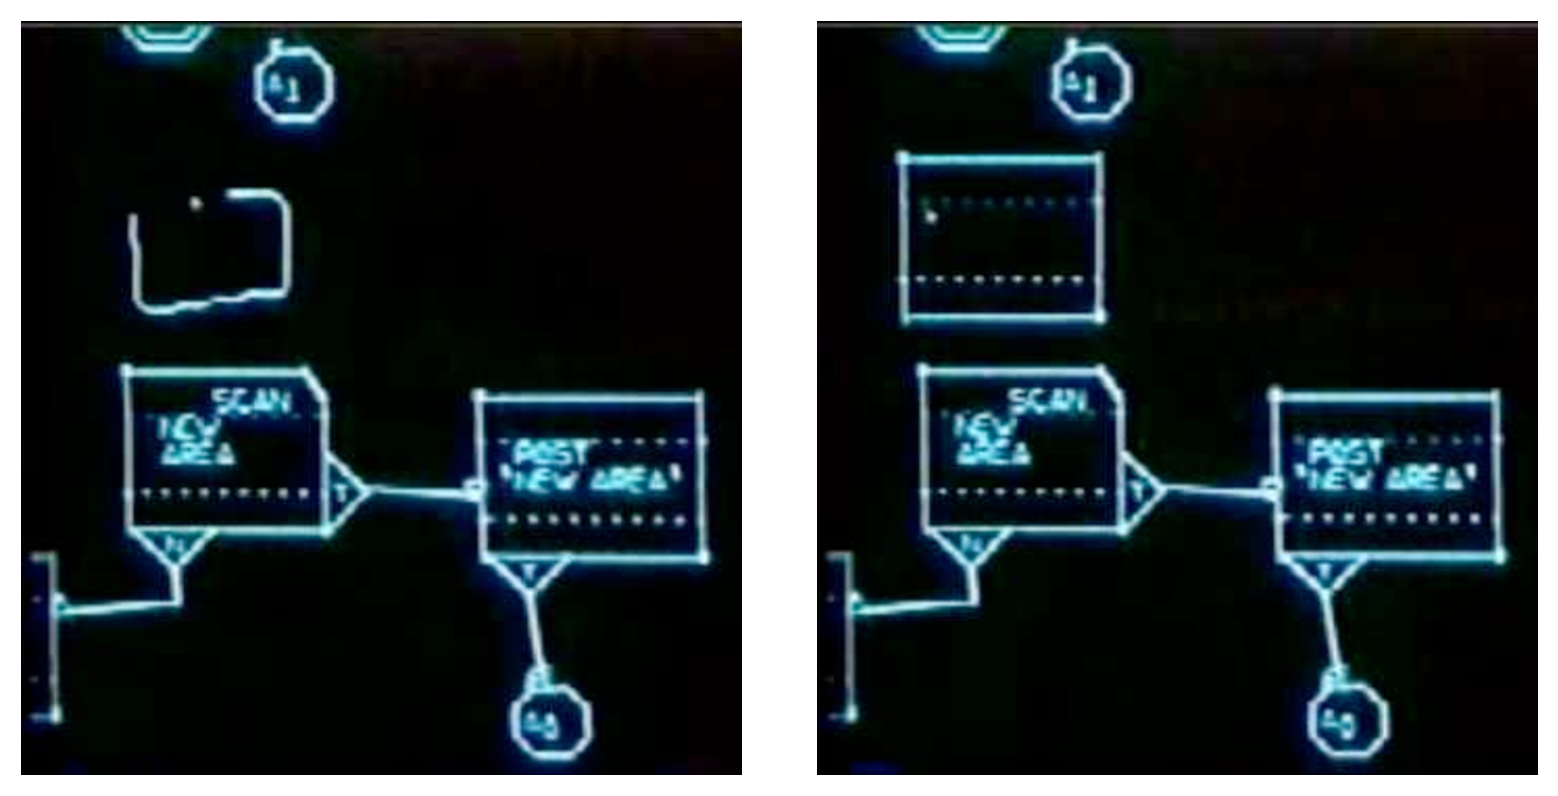
\includegraphics[angle=0, origin=c, width=3.0in]{img/grail-box.pdf} 
  \caption{On left, a GRAIL user draws a model element in place. At
  right, the rectified element is displayed as a box.}
\label{fig:grail-box}
\end{center}
\end{figure}
\begin{figure}
\begin{center}
  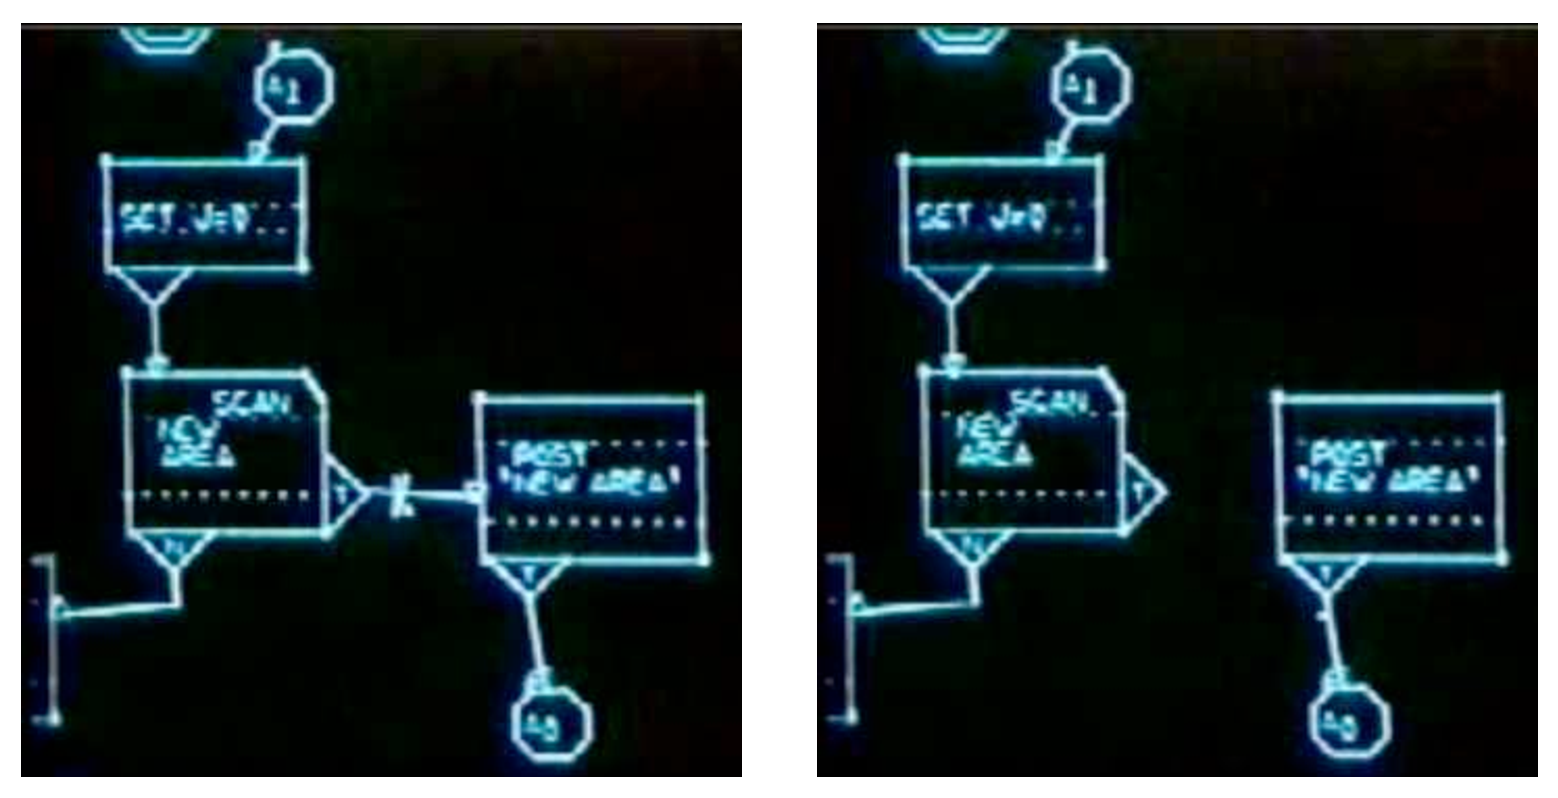
\includegraphics[angle=0, origin=c, width=3.0in]{img/grail-gesture.pdf}
  \caption{GRAIL's sketch interpretation is context sensitive. At left
  the user crosses out the connector, which is interpreted as a delete
  command, shown at right.}
\label{fig:grail-gesture}
\end{center}
\end{figure}
\end{samepage}

Alan Kay discussed Sketchpad and GRAIL in a 1986 lecture. A portion of
that talk is available on the Internet as part of the New Media
Reader~\cite{kay-sketchpad-grail-dynabook,nmr}. Kay shows video of
these pioneering systems and provides insightful commentary, reminding
viewers that much of the work in computer support for sketching has
roots from several decades ago.

There was no widely used pointing device until the Macintosh brought
about the mouse's widespread adoption in the mid-1980s. Owing to the
success of the mouse, pen and sketch based interaction was largely
ignored for years. This began to change when commercial pen computing
products came to market in the early 1990s, bolstered by the prospect
of interaction based on handwriting recognition. Companies such as GO
and GRiD developed and sold pen based tablet devices. IBM's early
ThinkPad computers (700T and 710T) were tablets. Yet these products
fared poorly, and by 1995 many pen computing ventures had gone out of
business. Pen computing did find a niche in the personal digital
assistant (PDA) market with devices such as the Apple Newton and
subsequently the more popular Palm Pilot. However, today's PDAs
typically favor on-screen keyboards over stylus input. Tablet PCs are
currently gaining popularity, primarily for making hand-written notes.

\section{Sketching challenges in HCI}
\label{sec:intro-hci-challenges}

The strength of sketching input lies in the speed and fluidity with
which people can express, interpret, and modify shapes and
relationships among drawn elements without necessarily attending to
details such as alignment or precise measurement. These strengths can
also be seen as the weaknesses of sketching. The equivocal, imprecise
nature of freehand drawing that so benefits humans is exactly why
machines have difficulty recognizing sketches.

Those who aim to create useful and usable systems based on sketch
recognition face a set of challenges including:
 
\begin{itemize}
\item Make hardware to support pen based interaction
\item Build comprehensive, robus toolkits for building sketch based
  systems
\item Create robust sketch recognition algorithms
\item Develop user friendly methods for training and modeling recognizable
 content
\item Design better interaction techniques for sketch based systems
\end{itemize}

This review elaborates on each of these challenges. Progress in one
area will likely require simultaneous work in others. For example, in
order to fully explore interaction design issues in recognition-based
interfaces, we first need sufficiently robust and accurate sketch
recognizers. In order to build recognizers capable of interpreting
sketches made by any person in any domain we must have methods for
modeling domain content. This in turn requires appropriate hardware
and interaction methods.

\section{Research themes in sketch based interaction}

This review details the primary themes of research shown in
Figure~\ref{fig:themes}: support for design, hardware, sketch
recognition, and human-computer interaction techniques. 

\begin{figure}
\begin{center}
  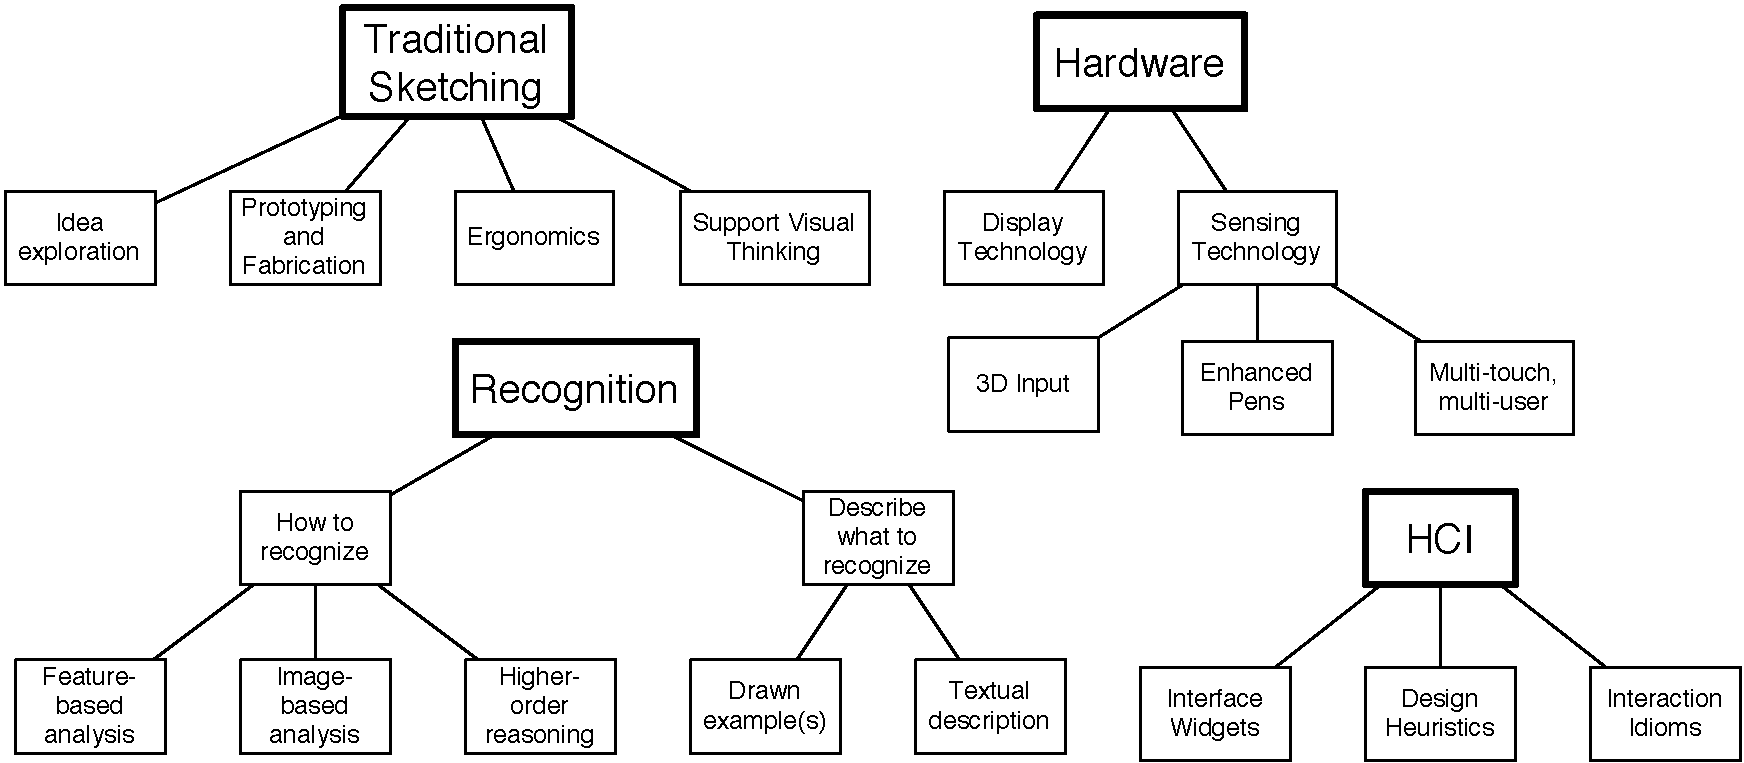
\includegraphics[angle=0,width=\linewidth]{img/themes-3-graffle.pdf}
  \caption{Research themes for sketch based interaction in design}
  \label{fig:themes}
\end{center}
\end{figure}

\textit{Traditional sketching:} (Section~\ref{sec:traditional})
Sketching plays a crucial role in the practice of design.  Sketching
helps designers think about problems and offers an inexpensive but
effective way to communicate ideas to others. The practice of
sketching is nearly ubiquitous: One recent study of interaction
designers and HCI practitioners found that 97\% of those surveyed
began projects by sketching~\cite{myers-behavior-design}. We must
understand the purpose and practice of sketching as it is done
\textit{without} computation if we hope to effectively support it
\textit{with} computation. Most research in computational support for
design sketching has focused on the \textit{early} phases when
designers are exploring high-level ideas. Fewer sketch based design
systems support \textit{later} stages of design when decisions must be
formalized. This section provides a basis for thinking about how, why,
and when (and when not) we may augment sketching with
computation. This discussion covers the cognitive affordances of
sketches and describes several empirical studies.

\textit{Hardware:} (Section~\ref{sec:hardware}) Physical devices
supporting pen based input have existed since RAND's digitizing tablet
was developed in the 1950s. Sensing technology (input) comes in many
forms. Sutherland's Sketchpad system in the early 1960s accepted input
from a light pen~\cite{sutherland-sketchpad}. Some devices promote
using fingers rather than pens, trading accuracy for convenience. Pen
based devices range in size from small (such as PDAs or ``pentop
computers'') to medium (Tablet PCs) to large (electronic
whiteboards). Other hardware considered by sketching researchers
includes electronic paper and ink. The device's size and means for
providing input dictate how and where it may be used, and how mobile
it is. New kinds of devices will lead to new ways of interaction.

\textit{Sketch recognition:} (Section~\ref{sec:recognition})
Recognition is central to many research systems in sketching. For this
reason, a large portion of this review is allocated to discussing
sketch recognition. Some drawn marks indicate domain elements, others
should be taken as commands, while others are annotations. As with
other recognition-based modes of interaction such as speech, sketch
based systems must have a model of what is to be recognized, as well
as algorithms for performing that recognition. Some recognition
techniques rely on input features such as corners, lines, and pen
speed. Other techniques compare the image formed by user input with
known elements. Still other techniques use artificial intelligence
methods such as Bayesian Networks for reasoning about likely sketch
interpretations. To recognize input the system must first have a model
of what may be recognized. Models are frequently made by drawing
examples. Other useful modeling strategies involve textual languages
describing the shape and relationships among visual elements.

\textit{Human-computer interaction:} (Section~\ref{sec:interaction})
User interfaces based on recognizing human speech, gestures, and
sketching pose interesting challenges for researchers in
human-computer interaction. New sketching input hardware, for example,
may promote new interaction styles or allow people to interact with
computers in new contexts, or collaborate in new ways. Because sketch
input may be ambiguous, the interface should not necessarily treat it
in the discrete, deterministic way that mouse and keyboard input is
treated. Further, resolving ambiguity may be delegated to the user,
which requires good interaction design.
